\chapter{Definitions/Terms}
\label{chap:definitions}

\subsubsection{Context} -
\subsubsection{Context Engine} The part of the program that handles context.
\subsubsection{Event} A single Windows Event Log event.
\subsubsection{Goroutine} A lightweight thread handled by the Go runtime.
\subsubsection{Log line} A single line of a dataset, which consist of a single event.
\subsubsection{Sysmon} A Windows service and driver that uses XML configuration files to enhance the log data given by Windows Event Log.
\subsubsection{Windows Event Log} A built-in mechanism in Windows that logs telemetry of what happens on the system. Can be enhanced by installing and configuring Sysmon on the system.
\subsubsection{Worker} -

\chapter{Datasets}
\label{chap:datasets}

\section{Evaluation of existing datasets?}

\subsection{Boss of the SOC}
\todo{Describe the BOTS-datasets}
\todo{Run some actual tests against the dataset to see if we get a hit with our rules}

\subsubsection{Version 1}
\url{https://github.com/splunk/botsv1}
\subsubsection{Version 2}
\url{https://github.com/splunk/botsv2}
\subsubsection{Version 3}
\url{https://github.com/splunk/botsv3}

\subsection{Mordor}
\url{https://github.com/hunters-forge/mordor}

\subsection{EVTX-ATTACK-SAMPLES}
\url{https://github.com/sbousseaden/EVTX-ATTACK-SAMPLES/}



\section{Mordor datasets}
The Mordor datasets are pre-recorded events generated by simulating adversarial techniques in a test environment using common red team tools like Empire and Cobalt Strike. The largest dataset in the collection aims to simulate a Advanced Persistent Threat (APT) known as APT3/Gothic Panda. The dataset contains two scenarios, both outlined in MITRE ATT\&CK Evaluation Operational Flow. The flow maps directly to MITREs ATT\&CK framework, by stepping through 10 different "steps".

\begin{enumerate}
\item Initial Compromise
\item Initial Discovery
\item Privilege Escalation
\item Discovery for Lateral Movement
\item Credential Access
\item Lateral Movement
\item Persistence
\item Collection
\item Exfiltration
\item Execution of Persistence
\end{enumerate}

The dataset contains approximately 100 000 log lines, and is made for security analysts to test their skills and tools using real known bad data.

\section{High signal, low noise dataset}
The concentrated dataset is a generated dataset that repeats the same 3 log lines that are enough to trigger a rule. The dataset is made in different sizes, from 1 000 lines, to 1 million lines.

This dataset is in no way "realistic", and is only used for performance testing when evaluating our real-time analysis throughput in a "worst case"-scenario setting.

\section{Low signal, high noise dataset}
This is the opposite of the highly concentrated dataset which contained the necessary log lines to repeatedly trigger a specific rule. This dataset only contains the nessessary events to trigger a single rule once, the rest of the events are simply background noise.

\section{Baseline dataset}
This dataset is a dataset with events that are all benign. This dataset is useful for measuring the speed at which the tools process and analyse the events, without triggering any rules.

\section{Dataset discussion}

\subsection{Are they realistic?}


\subsection{Are they representative?}
\subsubsection{Concentrated dataset}
The concentrated dataset is used strictly for measuring the performance of the systems in a worst-case scenario, and the dataset is in itself not representative of a real world scenario, ingesting log data that doesn't contain malice.

\subsubsection{Mordor datasets}
The Mordor datasets are not as concentrated and gathered from a test environment using realistic tools, techniques and procedures based on the MITRE ATT\&CK framework.



\chapter{Experiments}
\label{chap:experiments}

- Created a program that can parse log data in real time, and do correlation on the data..
- Implemented several versions that


Simple Event Correlator (SEC).
\section{Terminology}
\subsection{Context}
\subsubsection{Context Engine}

The context engine is 

\subsection{Worker}

A worker is a Goroutine that has the sole job of reading an event from a channel, trying to match the event to the given set of rules. If there is a match, the worker will decide if it has to 

\subsubsection{Goroutines}

A Goroutine is a lightweight thread that is managed by the Go runtime. it is not a thread in the traditional sense.


\section{Created a implementation that uses Simple Event Correlators own rule format (regex based)}

\subsection{SEC rule format}



\begin{lstlisting}
type=single
ptype=regexp
pattern=(\S+)sshd.*
desc=This is a description
\end{lstlisting}

\subsubsection{type}
Type of rule. There are many different types here.
I have focused on rules using "SingleWithThreshold" which takes an action if there are X number of matches in Y time.

Single

Suppress

Calendar

SingleWithSuppress

Pair

PairWithWindow

SingleWith2Thresholds

EventGroup

SingleWithScript

Jump

\subsubsection{ptype}
Pattern type. RegExp is a Perl regular expression. Can use variables.

SubStr

PerlFunc

Cached

TValue

\subsubsection{pattern}
The pattern that the log line will we tested against. The value of this pattern is based on the ptype. For example, if the ptype is set to "RegExp", the pattern will be a Perl regular expression.

\subsubsection{desc}
Description field. But used for defining "scopes" when correlating.

\subsubsection{action}
The action to take when the rule "hits".

\subsubsection{continue}

\subsubsection{context}

\subsection{Implementation}
As discussed in chapter X, the programming language Go was chosen for implementing our new program to analyze our datasets. I have chosen to only implement the SingleWithTreshold type, and the RegExp pattern type (ptype). The "SingleWithTreshold" type triggers an action if there are X number of matches within Y time. We consider this to be the most usable rule type for our purpose. For the pattern type, we choose to use "RegExp", which are Perl regular expressions. We consider this to be the best option for matching against syslog-based log lines.

Other than the fact that Go is a compiled language and Perl is a interpreted language, the main additions in our implementation is that our version:
\begin{itemize}
    \item Uses Go channels for re-injecting events into the context engine.
    \item The use of channels and goroutines gives us the ability to run in a threaded matter, utilizing multiple cores.
\end{itemize}

\subsubsection{Workers}
\todo{What are workers?}

\subsection{Results}
We want to see if our Go implementation can out-perform SEC when handling a high signal, low noise dataset. The following table shows the results for that:
\\
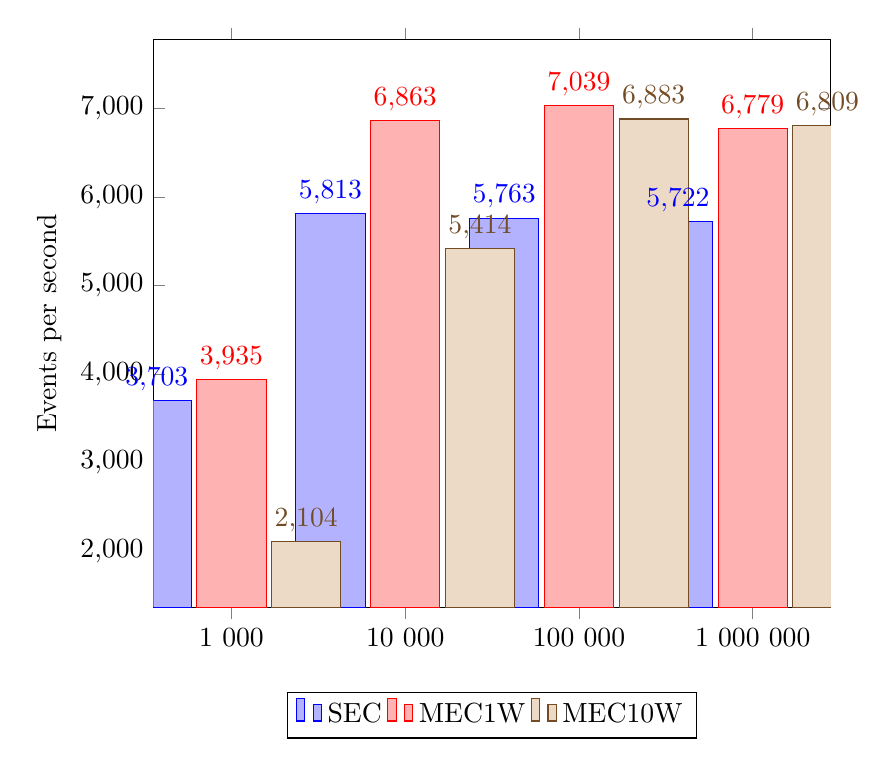
\begin{tikzpicture}
\begin{axis}[
    xtick=data,
	height=250pt,
	ylabel=Events per second,
	enlargelimits=0.15,
	legend style={at={(0.5,-0.15)},
	anchor=north,legend columns=-1},
	ybar,
	bar width=25pt,
	symbolic x coords={1 000, 10 000, 100 000, 1 000 000},
	nodes near coords,
	nodes near coords style={above}
]
\addplot coordinates {(1 000,3703) (10 000,5813) (100 000,5763) (1 000 000,5722)}; % SEC
\addplot coordinates {(1 000,3935) (10 000,6863) (100 000,7039) (1 000 000,6779)}; % MEC1W
\addplot coordinates {(1 000,2104) (10 000,5414) (100 000,6883) (1 000 000,6809)}; % MEC10W
\legend{SEC, MEC1W, MEC10W}
\end{axis}
\end{tikzpicture}
\\
These tests are run with 1 logical core on a "Intel(R) Core(TM) i7-7600U CPU @ 2.80GHz" (2 cores x 2 threads per core = max 4 logocal cores) and 24GB RAM.

\begin{itemize}
    \item Why is the MEC10W slower?
    \item Why are the runs on the 1 000 dataset generally lower?
\end{itemize}

By using all CPU cores available (4) instead of a single one, we can take better advantage of Gos concurrency model, and raise the throughput when using multiple workers and CPUs:

\pgfplotsset{scaled y ticks=false}
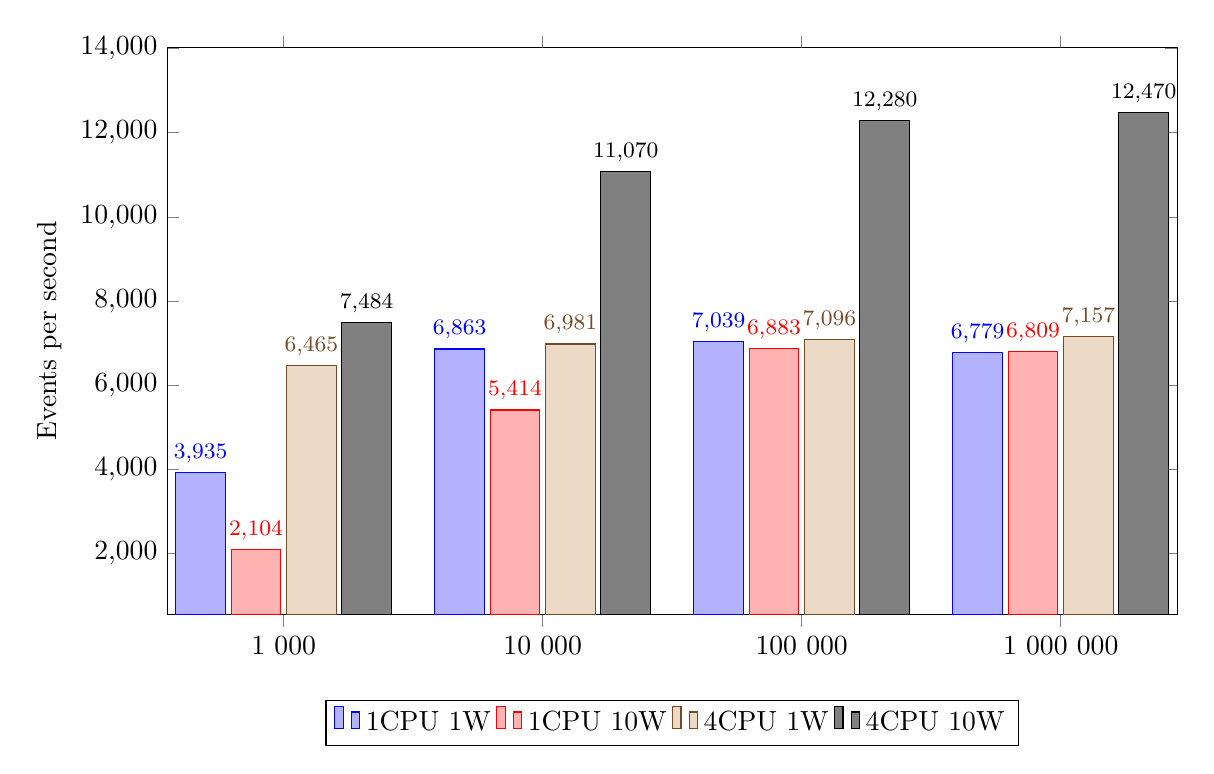
\begin{tikzpicture}
\begin{axis}[
    xtick=data,
    width=410pt,
	height=250pt,
	ylabel=Events per second,
	enlargelimits=0.15,
	legend style={at={(0.5,-0.15)},
	anchor=north,legend columns=-1},
	ybar,
	bar width=18pt,
	symbolic x coords={1 000, 10 000, 100 000, 1 000 000},
	nodes near coords,
	nodes near coords style={above, font=\footnotesize},
]
\addplot coordinates {(1 000,3935) (10 000,6863) (100 000,7039) (1 000 000,6779)}; % 1CPU 1W
\addplot coordinates {(1 000,2104) (10 000,5414) (100 000,6883) (1 000 000,6809)}; % 1CPU 10W
\addplot coordinates {(1 000,6465) (10 000,6981) (100 000,7096) (1 000 000,7157)}; % 4CPU 1W
\addplot coordinates {(1 000,7484) (10 000,11070) (100 000,12280) (1 000 000,12470)}; % 4CPU 10W
\legend{1CPU 1W , 1CPU 10W , 4CPU 1W , 4CPU 10W}
\end{axis}
\end{tikzpicture}

\begin{itemize}
\item Why is there a dip for 1CPU,10W when using a dataset of 1 000 events?
\item Why are the results of 1CPU,1W, 1CPU,10W and 10CPU,1W generally the same?
\item What can we say about 1CPU,10W "catching up" to the others around 100 000 events?
\end{itemize}

\section{Implemented a new rule format}
This format relies less on the extensive use of Regexes, as we saw in the rules used by Simple Event Correlator.

\subsection{Sigma}
\url{https://github.com/Neo23x0/sigma}

Sigma is an open standard for rules that are used to generically describe searches in log data. It is primarily used as a high-level rule that transcompile into SIEM queries like Splunk, ElasticSearch, QRadar, etc.

The rules are written in YAML (Yet Another Markup Language), and are key-value based.

\com{Testing}
\todo{Do somethiing}
\n{Testing note}
\begin{lstlisting}
title: Quick Execution of a Series of Suspicious Commands
id: 61ab5496-748e-4818-a92f-de78e20fe7f2
description: Detects multiple suspicious process in a limited timeframe
status: experimental
references:
    - https://car.mitre.org/wiki/CAR-2013-04-002
    - https://car.mitre.org/wiki/CAR-2013-04-003
author: juju4
modified: 2012/12/11
tags:
    - car.2013-04-002
logsource:
    category: process_creation
    product: windows
detection:
    selection:
        CommandLine:
            - ipconfig
            - arp
            - echo
    timeframe: 10s
    condition: selection | count() by MachineName > 3
falsepositives:
    - False positives depend on scripts and administrative tools used in the monitored environment
level: low
\end{lstlisting}

\subsection{Context}
\todo{What is context?}

\subsection{The Context Engine}
We are using a shared map between the "workers" of the application.

\subsection{Results}

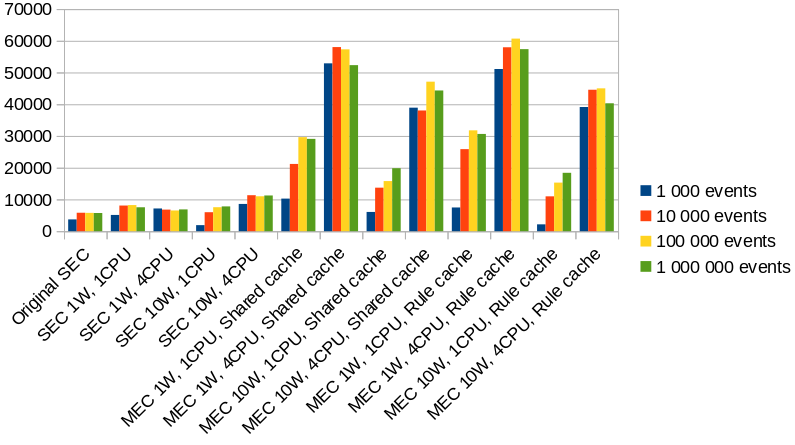
\includegraphics[scale=0.525]{figures/new-rule-format/performance.png}
\\
Min hypotese her, er at ved å bruke flere regler som trenger kontekst, så vil vi få et enda større sprang mellom shared og rule-based caching enn det vi ser over.
\\
Under har jeg generert 1000 regler og kjørt MEC på disse. Høyere søyle er bedre. Det er ganske tydelig at event-per-sekund her faller drastisk, da det må itereres over flere regler (2 vs 1000).
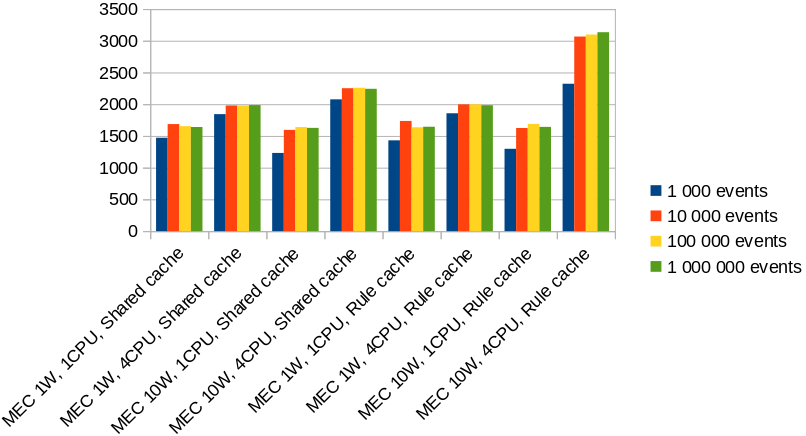
\includegraphics[scale=0.525]{figures/new-rule-format/performance-2.png}
\\
Som forventet så ser vi at rule-cache med 10W og 4CPU gir en 39.77\% økning sett opp imot 10W og 4CPU og shared caching.

Det som er interessant her er at det er liten forskjell mellom (1W, 1CPU), (10W, 1CPU) og (1W, 4CPU) mellom de forskjellige cache-typene. Dette gir mening, da lavt antall workers og CPU ikke drar ordentlig nytte av rule-based caching, og vil da falle ned til samme hastighet som shared cache.